
% \comentario{En general, las comillas hay que ponerlas angulares «», que también se llaman comillas españolas. Si decides no utilizar las españolas, no escribas '''' sino ``'' }
% Hoy en día es sencillo para cualquier persona con la suficiente motivación aprender a programar. De hecho, para programar en \textit{JavaScript} (ECMAScript) utilizando un entorno de ejecución como \textit{NodeJS} sobre un \textit{framework} como \textit{React}, ni siquiera necesitas conocimientos sobre \textit{hardware}, ni saber como se gestiona la memoria, ni hasta cierto punto la naturaleza de un ``puntero". Sin embargo, podríamos decir que estarías ``programando". Creo que cada vez es más accesible y tenemos más herramientas para poder plasmar nuestras ideas a través de la propia programación, y a la vez tanta abstracción nos aleja de la cantidad de pasos que hay detrás de cada línea de código.\\\\
% \comentario{No está claro que idea quieres transmitir y como está relacionada con el trabajo. Piensa en reescribirlo.}


% La primera vez que intente programar tenía trece años, e intente aprender \textit{Java} mediante unos tutoriales de \textit{Youtube}. En uno de los primeros vídeos, explicaba como se compila el código y las fases que atraviesa hasta convertirse en código máquina. Allí, lo explicaban de manera muy sencilla, primero tienes el código fuente, ese código se transforma en \textit{bytecode} (o código intermedio), y ese \textit{bytecode} pasa por una máquina virtual (JVM, Java Virtual Machine) para convertirse en código máquina. Resulta que el proceso de compilación me llamó la atención, y es por esto que he escrito mi propio ``mini''  lenguaje, al que he llamado GoneFSR, siguiendo las instrucciones y la estructura que propone David Beazley en su curso de BeGone, también me he basado en algunos capítulos del libro \cite{aho2006compilers} para tener un mayor entendimiento del análisis léxico y semántico. (estos dos parrafos tal vez haya que pasarlos a la introduccion)\\\\




El compilador está basado en el curso de David Beazley, en el que explica como desarrollado un compilador llamado \textit{BeGone}, sin embargo debido a algunas extensiones de este compilador que se han realizado además de la completa implementación de las funcionalidadas requeridas por el curso, he decidido llamarlo GoneFSR. \\\\
En las siguientes subsecciones analizaremos cada parte que componen este compilador frontend. Cuando compilas código en GoneFSR, el compilador pasa por varias etapas: análisis léxico, sintáctico, semántico, generación de código intermedio y generación de código llvm (Low Level Virtual Machine). Ese código llvm será traducido a un ejecutable por CLANG, como último paso.
\begin{figure}[h] 
    \centering
    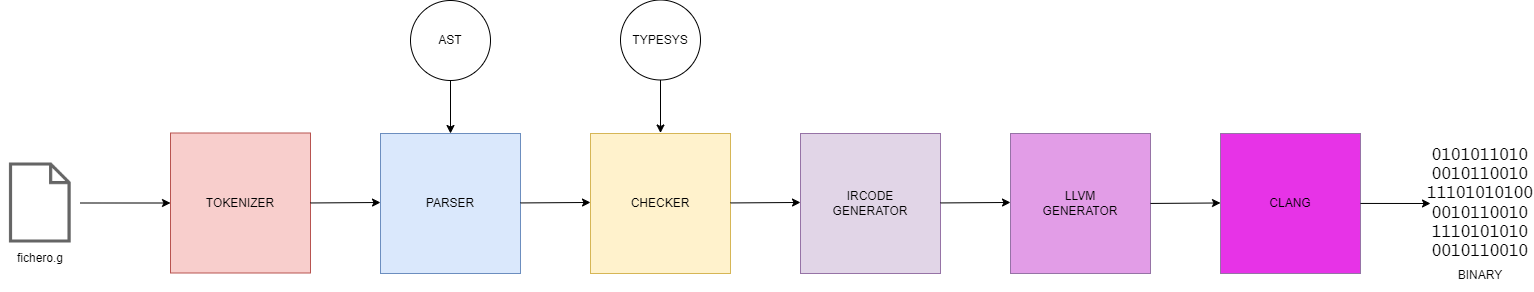
\includegraphics[width=1\textwidth,keepaspectratio]{img/compiler-schema.png}
    \parbox{\linewidth}{\centering Estructura de GoneFSR}
    \label{fig:mi_imagen}
\end{figure}
\section{Análisis léxico}
En un lenguaje cualquiera,  el léxico se entiende como el conjunto de palabras  que pertenecen a ésta.
Estas unidades mínimas con significado propio del lenguaje son lo que se denominan \textit{tokens}.
Al módulo del compilador, encargado del  \textit{tokenizado} o análisis léxico se le suele llamar \textit{Lexer}.
\subsection{Lexer}
La clase \href{https://github.com/domingoUnican/TFGPedroCastro/blob/main/code/compilerGoneFSR/gone/tokenizer.py}{Lexer} divide la cadena de caracteres de entrada (contenido del archivo ``.g'') en \textit{tokens}. Por \textit{token} se entienden todo tipo de palabra clave (\textit{keywords}), identificadores, literales, delimitadores como los paréntesis o el punto y coma. Aunque la función principal del \textit{Lexer} es generar tokens, también se encarga de ignorar algunos caracteres que no necesitamos que se traten como \textit{tokens} para que estos no pasen a la segunda fase, que sería el \textit{parsing} o análisis sintactico, un buen ejemplo de esto son los caracteres de salto de línea, o los comentarios. Para encontrar cada token recorre la cadena implementando un autómata finito que transiciona de estado en función del carácter que está recorriendo.\\\\
\begin{figure}[h] 
    \centering
    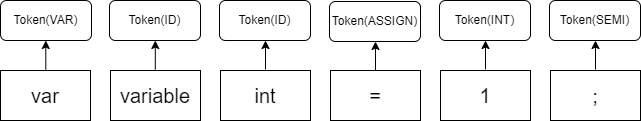
\includegraphics[width=0.8\textwidth,keepaspectratio]{img/tokens.png} .
    \label{fig:mi_imagen}
\end{figure}
\\\\
\subsubsection{Implementación}
Para abstraernos del código, explicaré lo esencial de la implementación del \textit{Lexer}. La clave está en las expresiones regulares, más conocidas como REGEX, permitiendo especificar que \textit{tokens} queremos encontrar sobre la entrada.\\\\
\noindent El orden en el que se definen los tokens tiene importancia, definir un token antes que otro en los que los dos comparten el comienzo del patrón, significa que se le dará prioridad al definido previamente, es por esto que todos los tokens del lenguaje se definen antes que los identificadores, ya que la REGEX de los identificadores engloba a palabras clave, como ``const'' o ``return''.\\\\
Los tipos de dato como \textit{int}, \textit{string} o \textit{char} son clasificados como tokens de tipo \textit{IDENTIFIER}, y más tarde durante la fase de análisis semántico serán validados, para que no se puedan definir variables con tipos arbitrarios.\\\\
Dominar las expresiones regulares es complejo, hay muchas reglas que debes conoces, muchas caracteres que dependiendo del contexto significan una cosa u otra: grupos de captura, contenedores, ``lookahead'' con condiciones, caracteres comodín, etc... \\\\
Describir el funcionamiento de estos, me llevaría probablemente otras diez páginas así que consideraré que con decir que es a través de estas expresiones regulares como capturamos los \textit{tokens}, es suficiente. Para que no queden sin explicar, pondré un ejemplo, sobre cómo distinguimos los enteros.
\begin{lstlisting}[style=pythonStyle]
INTEGER = r'0x[a-f0-9]+|0o[0-7]+|0b[10]+|d+'
\end{lstlisting}
\noindent Para aquellos entendidos en expresiones regulares, sabrán que hay un detalle que me he saltado sobre los enteros. Y es que un entero puede escribirse sobre diferentes bases, se puede escribir, en decimal, en binario, en octal y en decimal.
%\comentario{No les expliques a informáticos que son las diferentes bases, eso lo puedes dar por supuesto.}
En la expresión regular se puede distinguir que se define como un entero la cadena '0x' seguida de al menos un (símbolo +) carácter `a', 'b', 'c', 'd', 'e' y 'f' o de un dígito del cero hasta el nueve. Con esta configuración no se aceptaran como caracteres hexadecimales aquellos escritos con letras mayúscula, esto es una decisión arbitraria, ya que sería fácil admitirlos. Con el carácter '$|$' especificamos un 'or' en la expresión es decir que también pueden admitirse escritos en octal (comenzando con '0o' y seguidos de al menos un dígito del cero al siete), escritos en binario (comenzando con '0b' y seguidos de al menos un dígito del cero al uno), o escritos en decimal que es lo que quiere decir la subcadena 'd+', es decir al menos un dígito del cero al nueve. \\\\
Para cada uno de los \textit{tokens} del lenguaje hay una expresión regular que lo describe, para consultar todas las expresiones regulares, tenéis el código original en \href{https://github.com/domingoUnican/TFGPedroCastro/blob/main/code/compilerGoneFSR/gone/tokenizer.py}{tokenizer.pyº}.


\newpage
\section{Análisis sintáctico (\textit{parsing})}
Un \textit{token} no es nada por si solo, lo que lo define es como se relaciona con los otros \textit{tokens}. La definición de las relaciones entre tokens se le llama gramática.
\subsection{Tipos de datos}
En GoneFSR, hay cuatro tipos distintos de datos. 
\begin{itemize}
    \item{Números enteros (\textit{int}) de 32bits}
    \item{números decimales (\textit{float}): este tipo de dato normalmente se asocia a números de coma flotante 32 bits, pero en este lenguaje en la fase final de compilación se mapean a double (64 bits) en las instrucciones llvm}
    \item{carácter (\textit{char}):  es simplemente un único carácter estando permitidos cualquier letra o número, además de caracteres especiales como \textbackslash, \textbackslash n, \textbackslash ", \textbackslash xhh (siendo hh cualquier valor hexadecimal lo que permite representar cualquier carácter ASCII). Los calores \textit{char} en este lenguaje siempre tendrán que estar recogidos sobre comillas simples.}
    \item{cadenas de caracteres (\textit{strings}): son conjuntos de caracteres empezando y acabando por comillas dobles, pudiendo contener todo tipo de caracteres, escapados o no. Es importante decir que no se puede iterar sobre ellas. }\\ 
\end{itemize}
\subsection{Reglas básicas de la gramática}
\label{reglas gramaticales 1}
Todos las sentencias en GoneFSR, deben acabar en ``;", como por ejemplo en lenguajes como C, o Java. En este lenguaje existen variables mutables e inmutables, para las inmutables o constantes no es necesario especificar un tipo de dato ya que se infiere del propio dato.\\\\
La sintaxis para constantes sería
\begin{lstlisting}[style=goneStyle]
const ID = value;
\end{lstlisting}
En el caso de las variables mutables si se requiere que el usuario especifique un tipo de dato en concreto de los cuatro disponibles. La sintaxis sería
\begin{lstlisting}[style=goneStyle]
var ID datatype = value;
\end{lstlisting}

%\comentario{Como comentario, no hagas saltos de página. Esto hace que el texto quede más espaciado, dando mala impresión. Tampoco digas sobre la primera sentencia condicional, si no hay más sentencias condicionales.}
\noindent La sentencia condicional \textit{if}, se define con  una sintaxis ampliamente extendida entre otros lenguajes.

\begin{lstlisting}[style=goneStyle]
if (condition) {
    statements
}
\end{lstlisting}

\noindent Para escribir un ``if else''.

\begin{lstlisting}[style=goneStyle]
if (condition) {
    statements
}
else {
    statements
}
\end{lstlisting}

\noindent En caso de querer definir un bucle,
%\comentario{en vez de escribir, ¿definir? ¿describir? ¿utilizar un bucle?}
GoneFSR, tan solo cuenta con el bucle ``while"  por simplicidad, que se escribiría con la sintaxis.

\begin{lstlisting}[style=goneStyle]
while (condition) {
    statements
}
\end{lstlisting}

\noindent Ya solo nos queda por ver como se declaran las funciones. En GoneFSR las funciones se escriben tal que así.
\begin{lstlisting}[style=goneStyle]
func function_name (*arguments) return_datatype {
    statements
}
\end{lstlisting}
En GoneFSR, hay tres funciones \textit{built-in}, es decir las puedes llamar sin necesidad de importar nada, ``print",``coder'' y ``decoder". Estas funciones tienen una sintaxis especial, ya que no usan paréntesis para recoger sus argumentos. Por ejemplo, para usar la función ``coder''.
\begin{lstlisting}[style=goneStyle]
coder "<path-inputfile>" "<path-outputfile">;
\end{lstlisting}
\subsection{Tipos de operaciones}
Las operaciones binarias disponibles en el compilador tanto para enteros como para decimales son: suma, resta, multiplicación y división. Siguiendo el estándar cada una de ellos se asocia con los símbolos +, -, *, /, respectivamente.\\\\
El compilador cuenta con las siguientes operaciones condicionales para después con las sentencias condicionales (``\textit{conditional statements}'') poder  bifurcar el código, menor que ($<$), mayor que ($>$), menor o igual que ($\leq$), mayor o igual que ($\geq$), igual que (==) y no igual que (!=), todas estos operadores funcionan tanto para int como para float. Las comparaciones entre booleanos son las siguientes: igual que (==), no igual que (!=), ``y`` ($\And\And$) y ``o`` ($||$).\\\\
El símbolo + y -, también actúan como operadores unarios para int y float, para especificar cuando un número es positivo o negativo. Para lo booleanos existe el operador unario !, el cual sirve para negar el valor de la variables booleana. 
\subsection{Reglas avanzadas de la gramática}
\label{reglas gramaticales 2}
Puntualizaciones en la gramática de las funciones de GoneFSR. 
\begin{itemize}
    \item{Las funciones en GoneFSR siempre tienen que retornar un tipo de dato, ya que no existe el tipo de dato void como en C.}
    \item{Todos los flujos de una función deben retornar.}
    \item{No se permite definir funciones anidadas dentro de otras funciones.  }
    \item{No se permite redefinir funciones ya definidas.}
    \item{Ninguna variable ya sea mutable o inmutable puede tener como identificador el nombre de uno de los tipos del lenguaje.}
    \item{Todo código escrito fuera de una función se considera global y se ejecutará en una función especial ``\textit{premain}'' (inicialización de variables globales).}
    \item{Cada función tiene su propio \textit{scope}, por lo que cada función tiene su propia tabla de símbolos.}
    \item{No se pueden hacer cadenas con operadores de comparación como por ejemplo $0<=j<=5$, si no que la manera correcta de escribir lo mismo sería $0<=j \And\And j<=5$.}
    \item{Todo código escrito después de un \textit{return} se notificará como un error, ya que es código deprecado.}\\
\end{itemize}
%\comentario{No  es correcto decir evaluar el código como un error. ¿No cumple la especificación?}


 %\comentario{Esto piensalo si lo quieres decir, quizás fuera mejor proponerlo a trabajos futuros. (mover a trabajos futuros)}

\subsection{Parsing}
%\comentario{Esto no está ordenado, hay poca parte del análisis semantico (error checking), y si hay de la parte del sintactico.}


%\comentario{Esto va en la parte de análisis sintáctico, pero no debes decir que más adelante se explicará, se explica más adelante y punto.}
En el \textit{Parser} establecemos las reglas de nuestra gramática. Nos basaremos en la notación BNF (Backus Naur Formalism) para definir nuestra gramática libre de contexto. Una vez definida la gramática, el \textit{Parser} creará un AST (Abstract Syntax Tree) partiendo de los tokens generados por el \textit{Lexer}, esta es una estructura jerárquica en forma de árbol el cual representa las relaciones entre sentencias, expresiones y operadores como nodos.\\\\
Una gramática libre de contexto puede ser definida como una tupla $(V, \Sigma, R, S)$ donde $V$ es un conjunto no terminales, $\Sigma$ es un conjunto de símbolos terminales, $R$ es un conjunto de producciones o reglas que asocian cada no terminal a una cadena $s$ donde $s \in (V \cup \Sigma)*$. Y $S$ es un símbolo terminal perteneciente a $V$, que es el símbolo sobre el que se comienzan aplicar las reglas. En nuestra gramática libre de contexto $\Sigma$ son los tokens generados por el \textit{Lexer}. Los símbolos no terminales $V$ y las producciones son las que definirán nuestro lenguaje. \\\\
Representados en BNF los tres símbolos no terminales y sus reglas de producción asociadas de los que derivan todos los demás son (siendo \textit{program}, $S$):
\begin{align*}
    &\text{program} \rightarrow \text{statements | $\lambda$ }  \\
    &\text{statements} \rightarrow \text{statements statement | statements }  \\
    &\text{statement} \rightarrow \text{const\_declaration | var\_declaration | assign\_statement | if\_statement }  \\
     &\text{| while\_statement | return\_statement | print\_statement | coder\_statement | decoder\_statement }  \\
\end{align*}
Podéis consultar la gramática totalmente desarrollada en \ref{apéndice 1}. Esta gramática describe las reglas gramáticas básicas descritas previamente en esta sección. Es decir, partiendo de $S$ se va rellenando el AST hasta que se consigue una estructura que representa la estructura gramática del programa, esta técnica se le llama \textit{parsing} recursivo descendente.\\\\
En la práctica se definen funciones para cada regla gramatical y cada función llama a las reglas inferiores (funciones) hasta que se llega al nivel más bajo. En ese nivel se comparan los tipos de tokens si coincide, se acepta como el \textit{parsing} correcto. Si no, se retrocede en el nivel de reglas hasta que coincide con alguno de los tipos. Si el token no coincide con ninguno de los tipos se lanza un error.\\\\
%\comentario{No des comentarios personales en una memoria técnica o reducelos al mínimo posible. Intenta ir siempre al grano.}
\noindent Esta etapa se implementa en dos clases, una de ellas es la clase \href{https://github.com/domingoUnican/TFGPedroCastro/blob/main/code/compilerGoneFSR/gone/parser.py}{parser.py} que hereda directamente de la clase \textit{Parser} de SLY, y la otra clase, es la clase encargada de definir las clases de cada nodo del AST, \href{https://github.com/domingoUnican/TFGPedroCastro/blob/main/code/compilerGoneFSR/gone/ast.py}{ast.py}.
\newpage
\subsection{Precedencia}
 \textit{``A grammar can have more than one parse tree generating a given
string of terminals. Such a grammar is said to be ambiguous.''} de \cite{aho2006compilers}.\\\\
Es necesario definir una precedencia en el \textit{Parser} para que no haya ambigüedades a la hora de crear el AST. Ya que se pueden generar dos AST distintos pero igual de válidos para nuestra gramática: \\
\begin{figure}[h] 
    \centering
    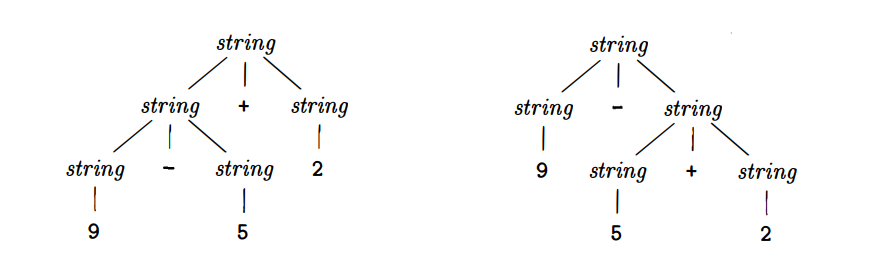
\includegraphics[width=0.8\textwidth,keepaspectratio]{img/astambiguos.png}
    \parbox{\linewidth}{\centering Ejemplo para 9 - 5 + 2 de \cite{aho2006compilers}}
    \label{fig:mi_imagen}
\end{figure}
\\\\
Para solucionar este problema definiremos la precedencia (que símbolo es evaluado primero) como una tabla en la que las filas están ordenadas de menor a mayor prioridad. En esta tabla habrá una tercera columna que será la asociatividad, que determina que operador es evaluado primero dentro del mismo rango de operadores.
\begin{center}
\begin{tabular}{ l c c }
 Nombre & Operadores & Asociatividad \\ \cline{1-3}
 Lógicos & ||, \&\&  & izquierda \\  d
 Comparación & $>,<$ & no asociativos \\
 Comparación 2 & $\leq, \geq, ==, \neq$ & izquierda \\
 Terms & $+, -$ & izquierda \\
 Factores & $*, /$ & izquierda \\
 Negación & $!$ & derecha
\end{tabular}
\end{center}
\newpage
\subsection{Clases nodos del AST}
Cada nodo del AST se representa por una clase, cada clase hereda de otra clase superior que clasifica el nodo entre cuatro posibles categorías: \textit{Statement} (sentencia), \textit{Expression}, \textit{Datatype} y \textit{Location}, este último se refiere a valores guardados en memoria como variables, constantes o funciones.
\begin{figure}[h] 
    \centering
    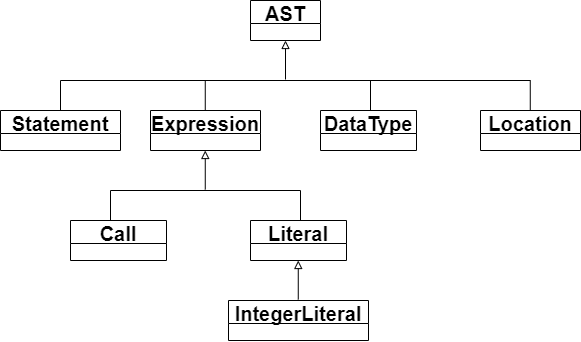
\includegraphics[width=0.8\textwidth,keepaspectratio]{img/astuml.png}
    \parbox{\linewidth}{\centering Diagrama UML parcial de la herencia entre nodos}
    \label{fig:mi_imagen}
\end{figure}\\
A la hora de definir los nodos lo importante es representar las asociaciones entre nodos con otros nodos. Por ejemplo el nodo ``ConstDeclaration'' tiene como atributos un nombre de tipo ``string'' y un valor de tipo ``Expression'', o el nodo ``BinOp'' (Binary Operation) que tiene como atributos el tipo de operación, el operando izquierdo, que será una instancia de la clase ``Expresssion'' y el operando derecho, otra instancia de esa misma clase.\\\\ 
Todo esto se entiende mucho mejor con un ejemplo de un AST de un programa en GoneFSR. Es un ejemplo muy sencillo, pero la idea creo que puede quedar clara con esto. Este sería el código fuente.

\begin{lstlisting}[style=goneStyle]
func main () int {
    var b int = 1;
    if 1 < 3 {
        b = 7;
        print b;
    }
    return 0;
}
\end{lstlisting}


\newpage Y este el AST asociado generado por el \textit{Parser} en base a ese código.
\begin{figure}[h]
    \centering
    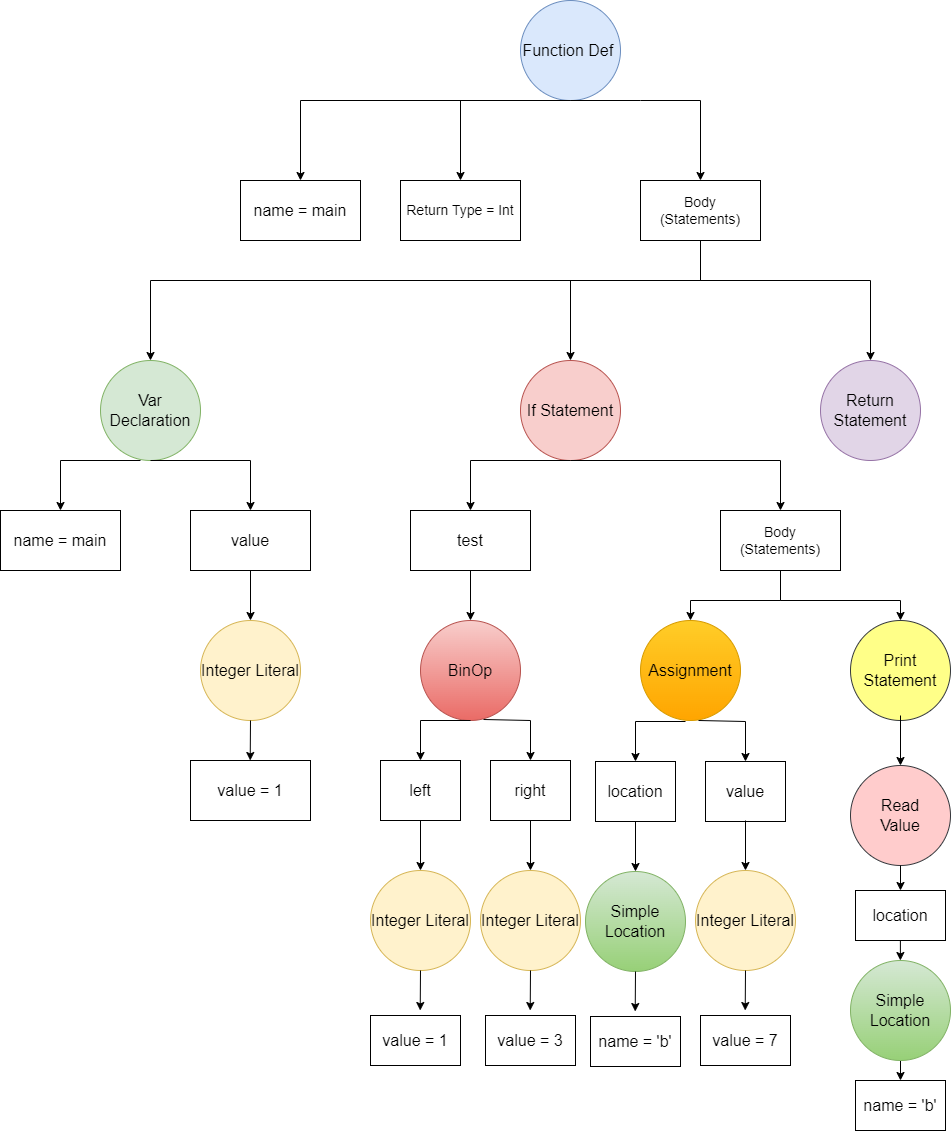
\includegraphics[width=0.9\textwidth,keepaspectratio]{img/asttree_latexexample.png} 
    \parbox{\linewidth}{\centering Ejemplo AST}
    \label{fig:mi_imagen}
\end{figure}

\newpage
\section{Análisis semántico}
El análisis semántico se asegura de que cada nodo del AST tengan sentido semántico. Una buena etapa de análisis semántico debe dar feedback al programador de las cosas que debe corregir para que su programa, al menos compile. Porque si el analizador semántico detecta que alguna expresión, declaración, inicialización o sentencia no tiene sentido lanzará un error, que prevendrá la generación de código. 
\subsection{Recorriendo el AST}
Las clases encargadas del análisis semántico y de la generación de código intermedio necesitan recorrer el árbol, para se capaces de realizar este recorrido heredan de una clase \textit{NodeVisitor} que está basada en una clase muy parecida del modulo de python \textit{ast.NodeVisitor}. Esta clase permite definir métodos asociados a cada tipo de nodo del árbol, los cuales a su vez contendrán llamadas a los métodos de los hijos de ese nodo. Esto provocará que de manera recursiva se recorran todos los nodos. Por ejemplo, que en una comparación se comparen 
 dos datos del mismo tipo.\\\\
En el caso del \textit{Checker}, clase encargada del análisis semántico, en cada método se define las carácteristicas que se quieren validar de ese nodo. 
\subsection{Funcionamiento \textit{Checker}}
La clase \href{https://github.com/domingoUnican/TFGPedroCastro/blob/main/code/compilerGoneFSR/gone/checker.py}{\textit{Checker}} cuenta con unas tablas de símbolos durante el análisis que le permiten recordar que símbolos han sido declarados, en mi implementación divido esta tabla de símbolos en tres subtablas: una tabla para símbolo globales, otra tabla para símbolos locales y una última tabla para las funciones. \\\\
A la hora de definir el método de un nodo, es importante el orden en el que visitas los nodos, ya que hay casos en los que se deben visitar primero los hijos, para después poder analizar los tipos de estos. Como en el caso de las operaciones binarias, que toman dos operandos como ``\textit{parametros}''. \\\\
En el caso de las localizaciones (``locations'') es necesario definir un atributo especial antes de visitar el nodo \textit{Location} para saber si se refieren al símbolo en modo escritura o lectura.\\\\
Cada vez que se visita un nodo de definición de una función el \textit{Checker} debe asegurarse de que la tabla de símbolos locales se vacíe para que los \textit{scopes} se respeten.
\subsection{Validaciones del análisis semántico}
El \textit{Checker} se encarga de que se cumplan todas las reglas gramaticales de la sección \ref{reglas gramaticales 2}, y además valida que no se incumplan ninguna de estas restricciones:
\begin{itemize}
    \item{ los símbolos estén definidos antes de que se les haga referencia, ya sea de lectura o de escritura, en el caso de variables mutables.}
    \item{Las valores asignados a variables mutables deben coincidir con el tipo declarado sobre estas.}
    \item{Las comparaciones siempre deben de ser entre valores del mismo tipo de dato, ya que en este lenguaje no existen los \textit{castings}.}
    \item{Si se intenta cambiar el valor de una constante, se notifica como error.}
    \item{No se nombre ningún símbolo con el nombre de un tipo de dato.}
    \item{Toda comparación debe resultar en un valor de tipo booleano.}
    \item{Se respeten los tipos de los parámetros de una función, ya que estos deben coincidir con los argumentos de una posible llamada a esta función}
    \item{Se respete la aridad (número de parámetros) de las funciones.}\\
\end{itemize}
En esta fase se realizan más validaciones, pero las listadas son las más relevantes.
\subsection{Validación de retorno de flujos en una función}
Me gustaría remarcar el sistema para controlar que todos los flujos de una función retornen, y en caso de que alguno de ellos no retorne lanzar un error / excepción. En una función se pueden dar dos casos, el primer caso es que la función cuente con un \textit{return} incondicional al final de la misma, por lo que el fallo estaría solventado. Y el segundo caso, en el que la función no cuenta con un \textit{return} al final de la misma, por lo que hay que verificar que cada uno de los flujos de la función terminan con el \textit{return} correspondiente. ¿Cómo podemos asegurarnos de que todos los flujos terminan? \\\\ 
En GoneFSR, el problema esta solucionado de la siguiente manera. Primero recorres uno a uno los statements del \textit{body} de la función y en caso de que haya un return, lo guardas como verdadero en una variable booleana; en caso de que no haya un return en el "main flow" de la función, ocurrirá lo siguiente, durante el recorrido de cada statement de la función cada vez que se ha pasado por una bifurcación del flujo ya sea un if, un if else o un while, se ha añadido un true o un false en una lista global. Al terminar de recorrer la función, te aseguras de que todos los booleanos de esa lista sean verdaderos, en caso contrario si ademas no se ha encontrado un ``return`` en el flujo principal salta el error. Último apunte, cada vez que se visita el nodo de una función evidentemente se vacía la lista global de booleanos.
\section{Generación de código intermedio}
En Python con el módulo \textit{dis} puedes conseguir el código intermedio de cualquier bloque de código. Estudiando este código puedes conseguir un entendimiento de como funciona realmente Python, entendiendo cosas como que Python debe evaluar un símbolo cada vez que se hace uso de este. La diferencia entre entender esos de detalles y no entenderlos, es la diferencia entre un buen programador y un mal programador, ya que estas cosas suelen tener un impacto significativo en el rendimiento de un programa. Este código intermedio tiene muchas similitudes y en ocasiones durante el desarrollo de esta parte del proyecto, me he fijado en que pasaría en Python en algunos casos en concretos para luego hacer lo mismo en mi compilador. \\\\
\noindent En este paso se suelen hacer cambios para que el código funcione en cualquier máquina. Un buen ejemplo es que a pesar de que en GoneFSR existen los booleanos, en este paso los booleanos se convierten en enteros ya que hay máquinas que pueden no contar con este tipo de dato. \\\\
En GoneFSR, nuestro código intermedio se parecerá al código intermedio de Python tan solo en forma, ya que nosotros trabajaremos con menos instrucciones y no haremos tantas optimización en tiempo de compilación. Además de que las instrucciones intermedias de Python (también se les llama bytecode) se interpretan directamente por la PVM (Python Virtual Machine), ya que en Python no se hace uso de llvm por cuestiones técnicas. 
\subsection{Transformación de AST en código intermedio}
(falta por explicar en detalle y con un ejemplo como funciona la clase encargada de la traduccion)Para definir el código intermedio de nuestro compilador, se ha escogido un estilo de código intermedio llamado \textit{Single Static Assignment} (SSA). Este paradigma se define por usar cada variable una sola vez. En la práctica esto implica que cada vez que se asigna un registro, se suma uno a un contador que a su vez es el índice del siguiente registro.Una instrucción de código intermedio puede tener los siguientes posibles argumentos: registros como operandos (``R'' + número, p.ej, ``R2''), caracteres (p. ej. para distinguir entre el tipo de comparación), y por último números enteros o flotantes. Ahora veamos la estructura de nuestras instrucciones de código intermedio.
\[ 
\texttt{ mnemónico argumento1, argumento2, \dots, argumentoN } 
\]
Existen instrucciones de manejo de memoria para cargar variables (LOAD) o almacenar valores en variables (\textsc{STORE}), entre ellas existe una distinción entre este tipo de instrucciones para variables locales y globales. También están contenidas en el código intermedio las instrucciones aritméticas y de comparación para tanto enteros como decimales. Por último, hay que mencionar a las instrucciones para crear bloques o bifurcaciones en el código. En el caso de funciones ``built-int`` (``print`` y ``fileToFSR`` cuentan con su propio mnemónico como se puede ver en el código [link a el codigo]).\\\\
Este módulo creará un diccionario con una lista de instrucciones de código intermedio para cada función. Ese diccionario se le pasará al generador de código llvm que será el encargado de dar el último paso para generar el ejecutable. 
\section{Generación de código LLVM}
\noindent LLVM es un conjunto de herramientas para el desarrollo tanto de frontend como de backend de compilación. Se define como frontend del compilador, el software encargado del análisis sintáctico o \textit{scanning}, el análisis semántico y de al menos generar una representación intermedia del código (en nuestro caso, la generación de código intermedio se hace en dos etapas). Por otro lado, el backend se define como la parte que optimiza y genera el código máquina optimizando y puliendo las instrucciones para que puedan ejecutarse en ese entorno en concreto. La ventaja más evidente de separar el proceso de compilado en estas dos etapas es que en lugar de hacer un compilador personalizado para cada lenguaje y para cada arquitectura, programas un compilador frontend para cada lenguaje y después un backend para cada arquitectura. Hay algunos compiladores que realizan las dos etapas como por ejemplo \textit{gcc}.
\subsection{De código intermedio a código LLVM}
(explicar aqui en detalle como funciona la clase encargada)
\subsection{Ejemplos llvm}
Veamos un ejemplo básico de uso del modulo \textit{llvm} para escribir código intermedio llvm. Siendo el código de python.
\begin{lstlisting}[style=pythonStyle]
from llvmlite.ir import Module, Function, FunctionType, IntType, IRBuilder, Constant, DoubleType, GlobalVariable, VoidType
import llvmlite.binding as llvm

# Inicializacion clases llvm
mod = Module('ejemplo')
main = Function(mod, FunctionType(IntType(32), []), name="main")
block = main.append_basic_block('entry')
builder = IRBuilder(block)

# Inicializacion variable global
global_operando = GlobalVariable(mod, IntType(32), 'globalop')
global_operando.initializer = Constant(IntType(32), 10)
valor_global_operando = builder.load(global_operando)
# Inicializacion variable local
local_operando = builder.alloca(IntType(32), name="localop")
builder.store(Constant(IntType(32), 5), local_operando)
valor_local_operando = builder.load(local_operando)
# calculo de resultado
resultado = builder.add(valor_local_operando, valor_global_operando, "resultado")
builder.ret_void()
print(str(mod))
\end{lstlisting}
Y el código llvm que obtenemos una vez ejecutamos el \textit{script} en Python es este.
\begin{lstlisting}[style=pythonStyle]
; ModuleID = "ejemplo"
target triple = "unknown-unknown-unknown"
target datalayout = ""

define i32 @"main"()
{
entry:
  %".2" = load i32, i32* @"globalop"
  %"localop" = alloca i32
  store i32 5, i32* %"localop"
  %".4" = load i32, i32* %"localop"
  %"resultado" = add i32 %".4", %".2"
  ret void
}

@"globalop" = global i32 10
\end{lstlisting}
El código llvm es bastante ofuscado e incómodo de leer, pero es portable. Esto tiene que ver con lo mencionado anteriormente del frontend y el backend en un compilador. Ahora que tenemos el código intermedio cualquier backend ya sea llc (el backend más común para llvm), clang, o incluso el propio compilador del lenguaje Rust (la gestión de memoria de este lenguaje merecería un TFG entero).\\\\
Vamos a analizar línea a línea que está pasando en ese código llvm. Lo primero de todo, el sitio donde definimos el código se le llama módulo y se podría entender como un ``fichero``. Dentro del módulo se definen funciones, y dentro de estas funciones se definen bloques. Estos bloques son la clave a la hora de implementar sentencias condicionales, ya que nuestro código deberá saber a que bloque debe ``saltar`` (hay algunos detractores en esto de dar saltos por el código, argumentan que dar saltos en memoria puede ralentizar el tiempo de ejecución).\\\\ Ya tenemos nuestro módulo, nuestra función y nuestro bloque donde escribir código. Bien, la siguientes dos instrucciones en el script de Python inicializan una constante, si ahora nos fijamos en el código llvm, podemos ver que la constante inicializada se encuentra fuera del \textit{scope} de la función main. La siguiente línea carga el valor de la constante en una variable temporal (\%``.2'').  Después se declara una variable local como \textit{int}, a esta variable se le da un valor de 5. Ahora i32 tiene un asterisco (*) detrás esto denota que actúa como puntero lo cual tiene sentido es decir estamos guardando un entero de 32 bits en la posición de memoria de ``localop''. Cargamos el valor de ``localop'' en otra variable temporal, para luego sumar ambas variables temporales guardando la suma en una variable local con nombre "resultado".
\\\\
Como al generador de codigo llvm le llega el código intermedio de la etapa anterior dividido en un diccionario (o HashMap, lo llamo diccionario porque así se le llama en Python), en el que las llaves son el nombre de las funciones. Creará en el modulo llvm tantas funciones como se le pasen por parámetro en la forma de esta estructura de datos. Sabiendo esto y que este generador utiliza los bloques de las funciones para escribir los saltos condicionales creo que lo correcto es finalizar la sección con el código llvm de la función \textit{main} de la sección 2.3.
\begin{lstlisting}[style=pythonStyle]
define i32 @"main"()
{
entry:
  call void @"premain"()
  %"b" = alloca double
  store double              0x0, double* %"b"
  store double 0x3ff0000000000000, double* %"b"
  %"R2" = load double, double* %"b"
  %"R4" = fcmp olt double %"R2", 0x4008000000000000
  br i1 %"R4", label %"B1", label %"B2"
B1:
  %"R7" = fadd double 0x401c000000000000, 0x4020000000000000
  store double %"R7", double* %"b"
  %"R8" = load double, double* %"b"
  call void @"_print_float"(double %"R8")
  br label %"B2"
B2:
  ret i32 0
}
\end{lstlisting}
La llamada a \textit{premain} es porque como ya comente todo código escrito fuera de \textit{main} se ejecute en \textit{premain} en este caso no hay código fuera de \textit{main} así que la función está vacía (el código llvm es en realidad, un poco más largo). \\\\
%La opción de no permitir código fuera de \textit{main} era igual de válida pero yo decidí implementarlo así arbitrariamente. 
Lo último que me queda por explicar es la traducción del \textit{if}, esto se hace a través de la intruccion ``br`` que si os fijáis es de tipo ``i1``, un integer de un solo bit, que es lo mismo que un booleano. Los otros dos términos de la instrucción son instrucciones label con dos etiquetas distintas ``B1`` y ``B2``. Pues bien si ese entero de un solo bit es 1 se saltará al bloque ``B1`` y en caso contrario a ``B2``. El valor de ese entero se determino en la operacion de comparación que se guarda en el registro temporal R4.

\section{Código llvm a código máquina}
CLANG actúa como backend de compilación en nuestro proyecto, ya que yo no he implementado las etapas de backend, generar el código máquina en función de la arquitectura o la etapa de enlazado. Hay que resaltar que CLANG emplea las librerías internas de LLVM para poder realizar el procecso de backend, ya que el propósito de CLANG es actuar de frontend, pero en este caso esa utilidad no nos hace falta. \\\\
En la práctica, tan solo tendremos que llamar al compilador desde la terminal y pasarle como argumentos tanto el archivo con el código intermedio llvm, como el archivo con las funciones ``built-in``, \href{https://github.com/domingoUnican/TFGPedroCastro/blob/main/code/compilerGoneFSR/gone/gonert.c}{gonert.c}. Con estos requisitos CLANG, nos escribirá un ejecutable en el directorio donde hayamos ejecutado el comando que será, en efecto nuestro programa.
\section{Implementación función fsr}
Para implementar las funciones de codificación y decodificación del formato de archivo de la sección \ref{formato archivo nlfsr}. Ha sido necesario hacer las siguientes modificaciones en el compilador.
\begin{enumerate}
    \item \textbf{Añadir token \textit{string}}: GoneFSR no contaba con datos \textit{string} así que hubo que añadir en el \textit{Lexer} un token de tipo \textit{string}.
    \item \textbf{Añadir keywords \textit{coder} y \textit{decoder}}: para identificar las nuevas funciones fue necesario añadir estas dos \textit{keywords} al \textit{Lexer}.
    \item \textbf{Nuevas clases de nodo del AST}: escribir una nueva clases para las sentencias \textit{coder} y \textit{decoder}, ambas heredaran de la clase \textit{Statement}. También tendrán las dos como atributos tanto el input path como el output path de los archivos que quieran usar como argumentos.
    \item \textbf{Cambios en el \textit{Parser}}: introducir nuevas reglas gramaticales para estas dos nuevas funciones.
    \item \textbf{Análisis semántico}: en la fase de análisis semántico obligar a que los parametros de las dos funciones sean del tipo \textit{string}.
    \item \textbf{Código intermedio}: crear instrucciones de código intermedio para las dos nuevas funciones, además las instrucciones de código intermedio para trabajar con strings (LOAD, STORE y MOV).
    \item \textbf{Compilación e instalación de los ejecutables \textit{coder} y \textit{decoder}}: Para ejecutar estas funciones es necesario instalar dos ejecutables en el sistema, la ruta correcta para instalarlos es \textit{``/usr/local/bin''}.
    \item \textbf{Escritura de las funciones en la librería nativa \textit{gonert.c}}: Al igual que las funciones para impirimir caracteres, enteros y flotantes. También será necesario crear tanto una función para imprimir strings como una función para el \textit{coder} que llame al ejecutable del sistema con los parámetros adecuados y una función igual para el \textit{decoder}.
    \item \textbf{Generación código llvm}: investigar y analizar el tratamiento de strings en llvm, y el paso de strings como argumento a funciones. Por último, añadir las nuevas funciones ``built-in'' al módulo llvm al igual que sus correspondientes métodos para generar el código llvm correspondiente.\\
\end{enumerate}
Si bien no es la mejor de las maneras para implementar una función nativa en un lenguaje ya que llamar a un ejecutable desde la propia función no es lo más común (aunque esto se intenta aliviar con la función \textit{execlp} de la librería estándar \textit{unistd.h} que sustituye el proceso original). Es una implementación funcional en un proyecto didáctico.\\\\
La mejor manera de implementar esto probablemente hubiera sido traspasar el código de las funciones de decodificación y codificación de Python y transpilarlo a C. Esto se puede conseguir con herramientas como \textit{Cython}, ha habido intentos de transpilar el código pero requería un afinamiento manual que traspasaba la escala del proyecto.\\\\
Tenéis en el repositorio una utilidad que instala los dos ejecutables en \textit{``/usr/local/bin''} para que no haya ningun problema en el uso de GoneFSR, [link a la utilidad].
\section{Testing del compilador}
Utilizando el modelo incremental iterativo, se han hecho pruebas para cada paso en el desarrollo del compilador. Y se han desarrollado en orden cada una de las fases para poder corregir fases anteriores si se produjesen errores.
\\
\subsubsection{Procedimiento}
Para cada etapa del compilador, el curso contaba con tests para probar la funcionalidad más básica de cada una de estas etapas, podéis consultar estos en \href{https://github.com/domingoUnican/TFGPedroCastro/tree/main/code/compilerGoneFSR/Tests}{tests}. Sin embargo, esta batería de tests no cubría todos los casos en los que el compilador debía de ser probado así que desarrolle mi propio conjunto de tests, el cual se encuentra en el directorio \href{https://github.com/domingoUnican/TFGPedroCastro/tree/main/code/compilerGoneFSR/Tests}{\textit{custom tests}}.

\subsubsection{Automatización de pruebas}
En el directorio \href{https://github.com/domingoUnican/TFGPedroCastro/tree/main/code/compilerGoneFSR/automation-scripts}{automatización de testing} podéis encontrar algunos \textit{scripts} escritos en \textit{bash} para crear dos archivos distintos, uno con la salida a distintos archivos de tests del compilador dado como ejemplo en el curso, el cual también tenéis en el directorio \href{https://github.com/domingoUnican/TFGPedroCastro/tree/main/code/compilerGoneFSR/goner}{compilador ejemplo}, y otro archivo en el cual escribía la salida de mi compilador. Utilizaba la comparación de estos dos archivos para saber si mi compilador estaba obteniendo los resultados correctos.
